\begin{figure}
\begin{fullwidth}
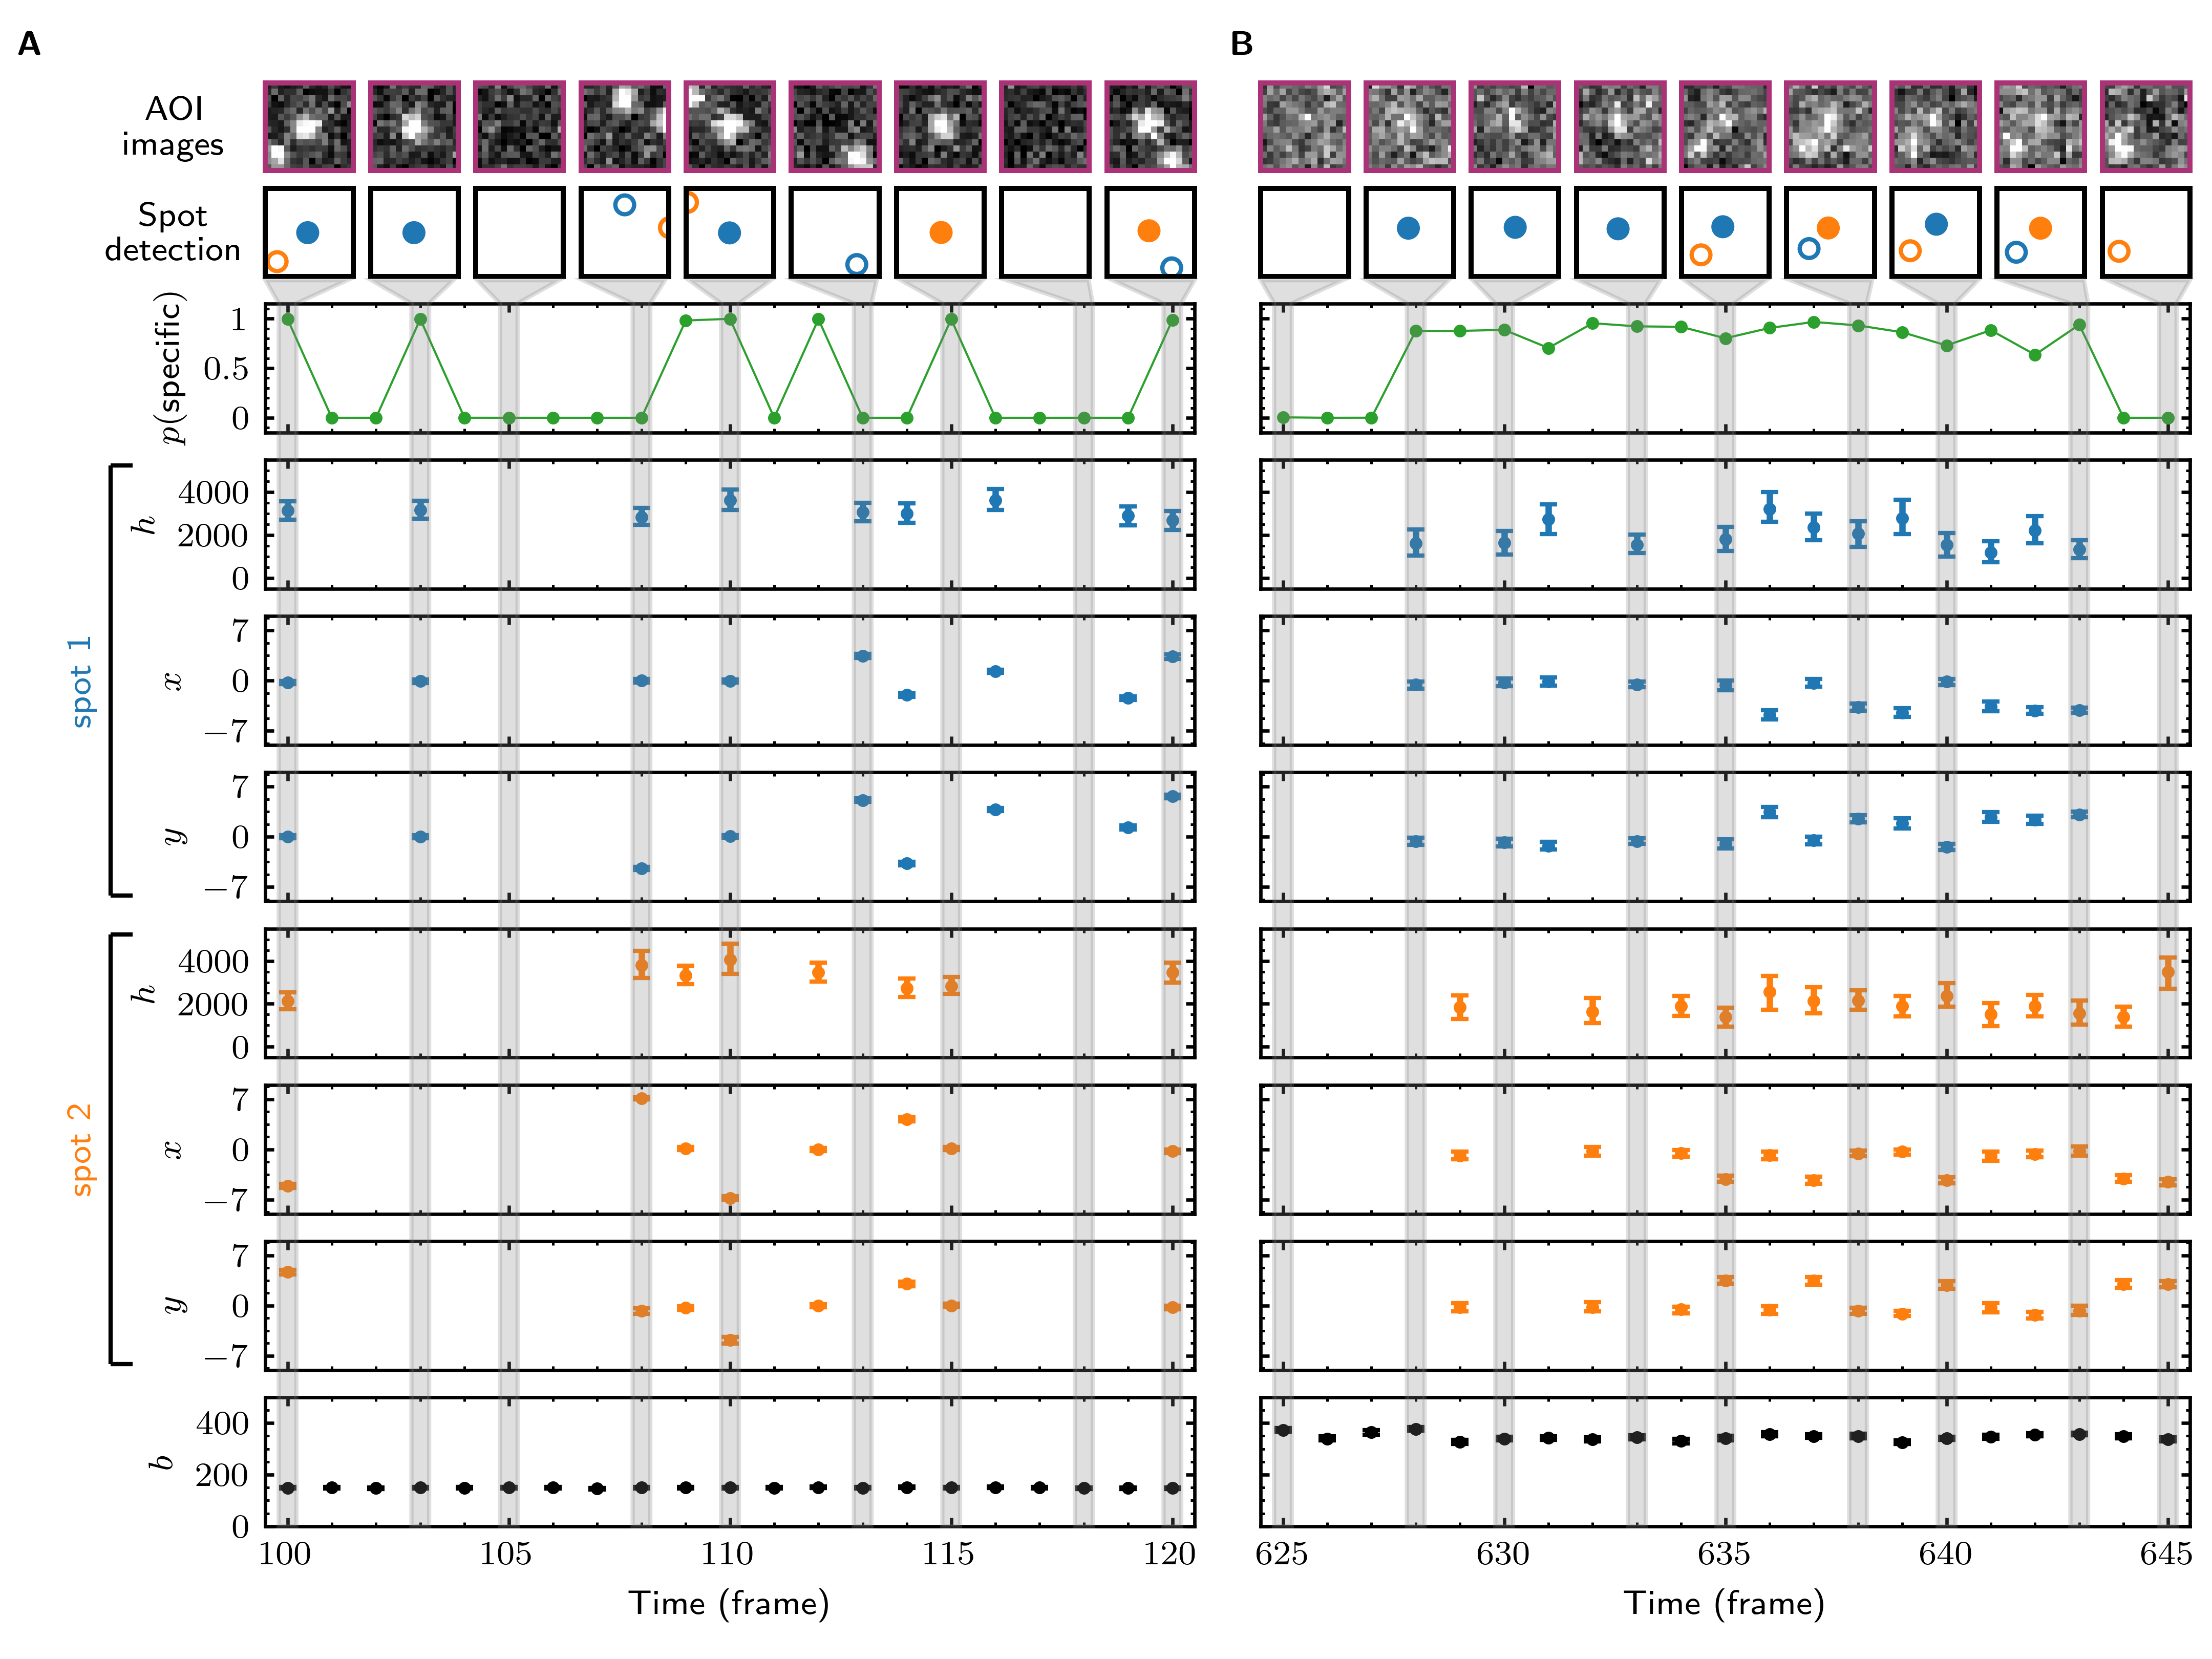
\includegraphics[width=183mm]{figures/tapqir_analysis.png}
\caption{\textbf{Tapqir analysis and inferred model parameters.} (\textbf{A},\textbf{B}) Tapqir was applied to simulated data (\texttt{lamda0.5} parameter set in Supplemental Data 1) (\textbf{A}) and to experimental data (Data set A in \TABLE{datasets}) (\textbf{B}). (\textbf{A}) and (\textbf{B}) each show a short extract from a single target location in the data set. The first row shows AOI images for the subset of frames indicated by gray shaded stripes in the plots; image contrast and offset settings are consistent within each panel. The second row shows the locations of spots determined by Tapqir. Spot numbers 1 (blue) and 2 (orange) are assigned arbitrarily and may change from fame to frame. For clarity, only data for spots with a spot probability $p(m=1) > 0.5$ are shown. Spots predicted to be target-specific ($p(\theta=k)>0.5$ for spot $k$) are shown as filled circles. The topmost graphs (green) show the calculated probability that a target-specific spot is present ($p(\mathsf{specific})$) in each frame.  Below are the calculated spot intensities ($h$), spot widths ($w$), and locations ($x$, $y$) for spot 1 (blue) and spot 2 (orange), and the AOI background intensities ($b$).  Again, for clarity data are only shown for likely spots ($p(m=1) > 0.5$). Error bars: 95\% CI (credible interval) estimated from a sample size of 500.  Some error bars are smaller than the points and thus not visible.}
\label{fig:tapqir_analysis}

\figsupp[Calculated spot probabilities.]{\textbf{Calculated spot probabilities. } The data sets used for panels A and B are identical to those in  \FIG{tapqir_analysis} A and B; the first two rows and the  $p(\mathsf{specific})$ (green) graph are reproduced from that figure. Blue graphs show the probability of being present ($p(m=1)$) and of being target-specific ($p(\theta=1)$) for the arbitrarily designated spot 1 in each frame.  Orange graphs show the analogous quantities $p(m=1)$ and $p(\theta=2)$ for spot 2. For a given image, the probability $p(\mathsf{specific}) \equiv p(z=1)$ that any target-specific spot is present is equal to $p(\theta=1) + p(\theta=2)$.}{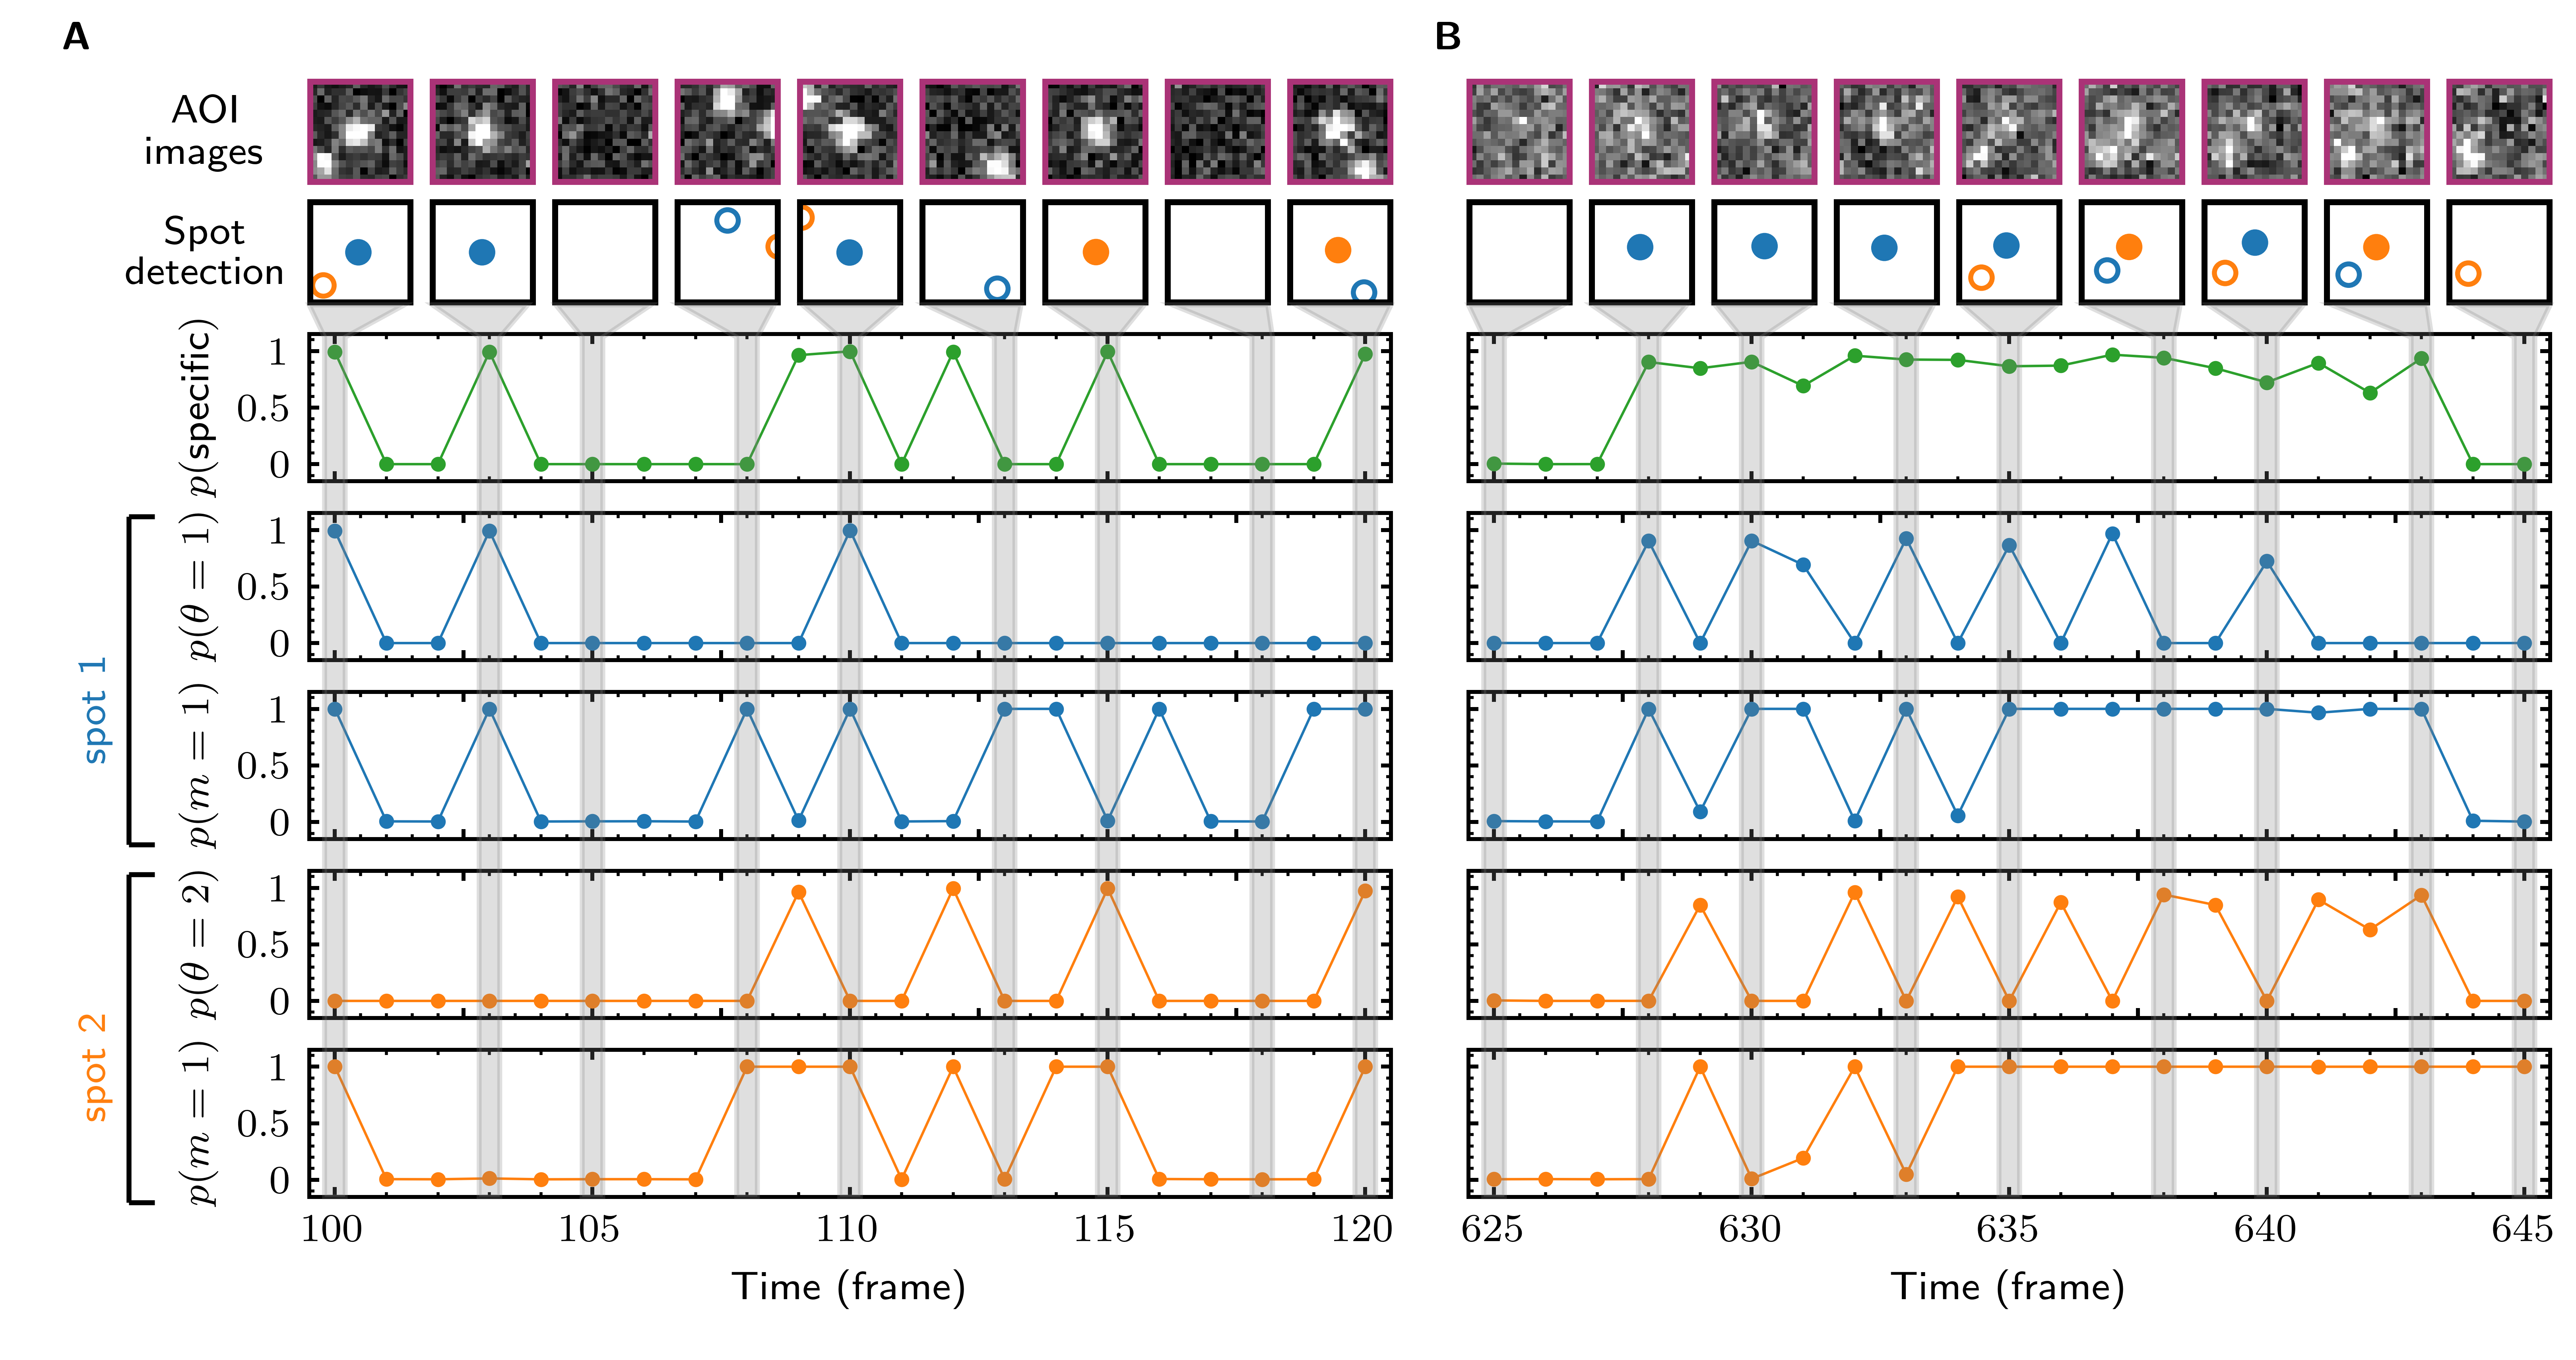
\includegraphics[width=183mm]{figures/tapqir_analysis_probs.png}}\label{figsupp:probs}

\figsupp[Reproduction of experimental data by posterior predictive sampling.]{\textbf{Reproduction of experimental data by posterior predictive sampling.} Example frames are shown from Data set A  (\textbf{A}: SNR = 1.61), Data set B (\textbf{B}: SNR = 3.77), Data set C (\textbf{C}: SNR = 4.23), and Data set D (\textbf{D}: SNR = 3.06) in \TABLE{datasets}. In each panel the top row shows AOI images selected from the experimental data and middle row shows corresponding images obtained by sampling from the posterior distributions. Image contrast and offset are consistent within each panel. The bottom row shows pixel intensity distributions from the experimental and posterior prediction images shown.}{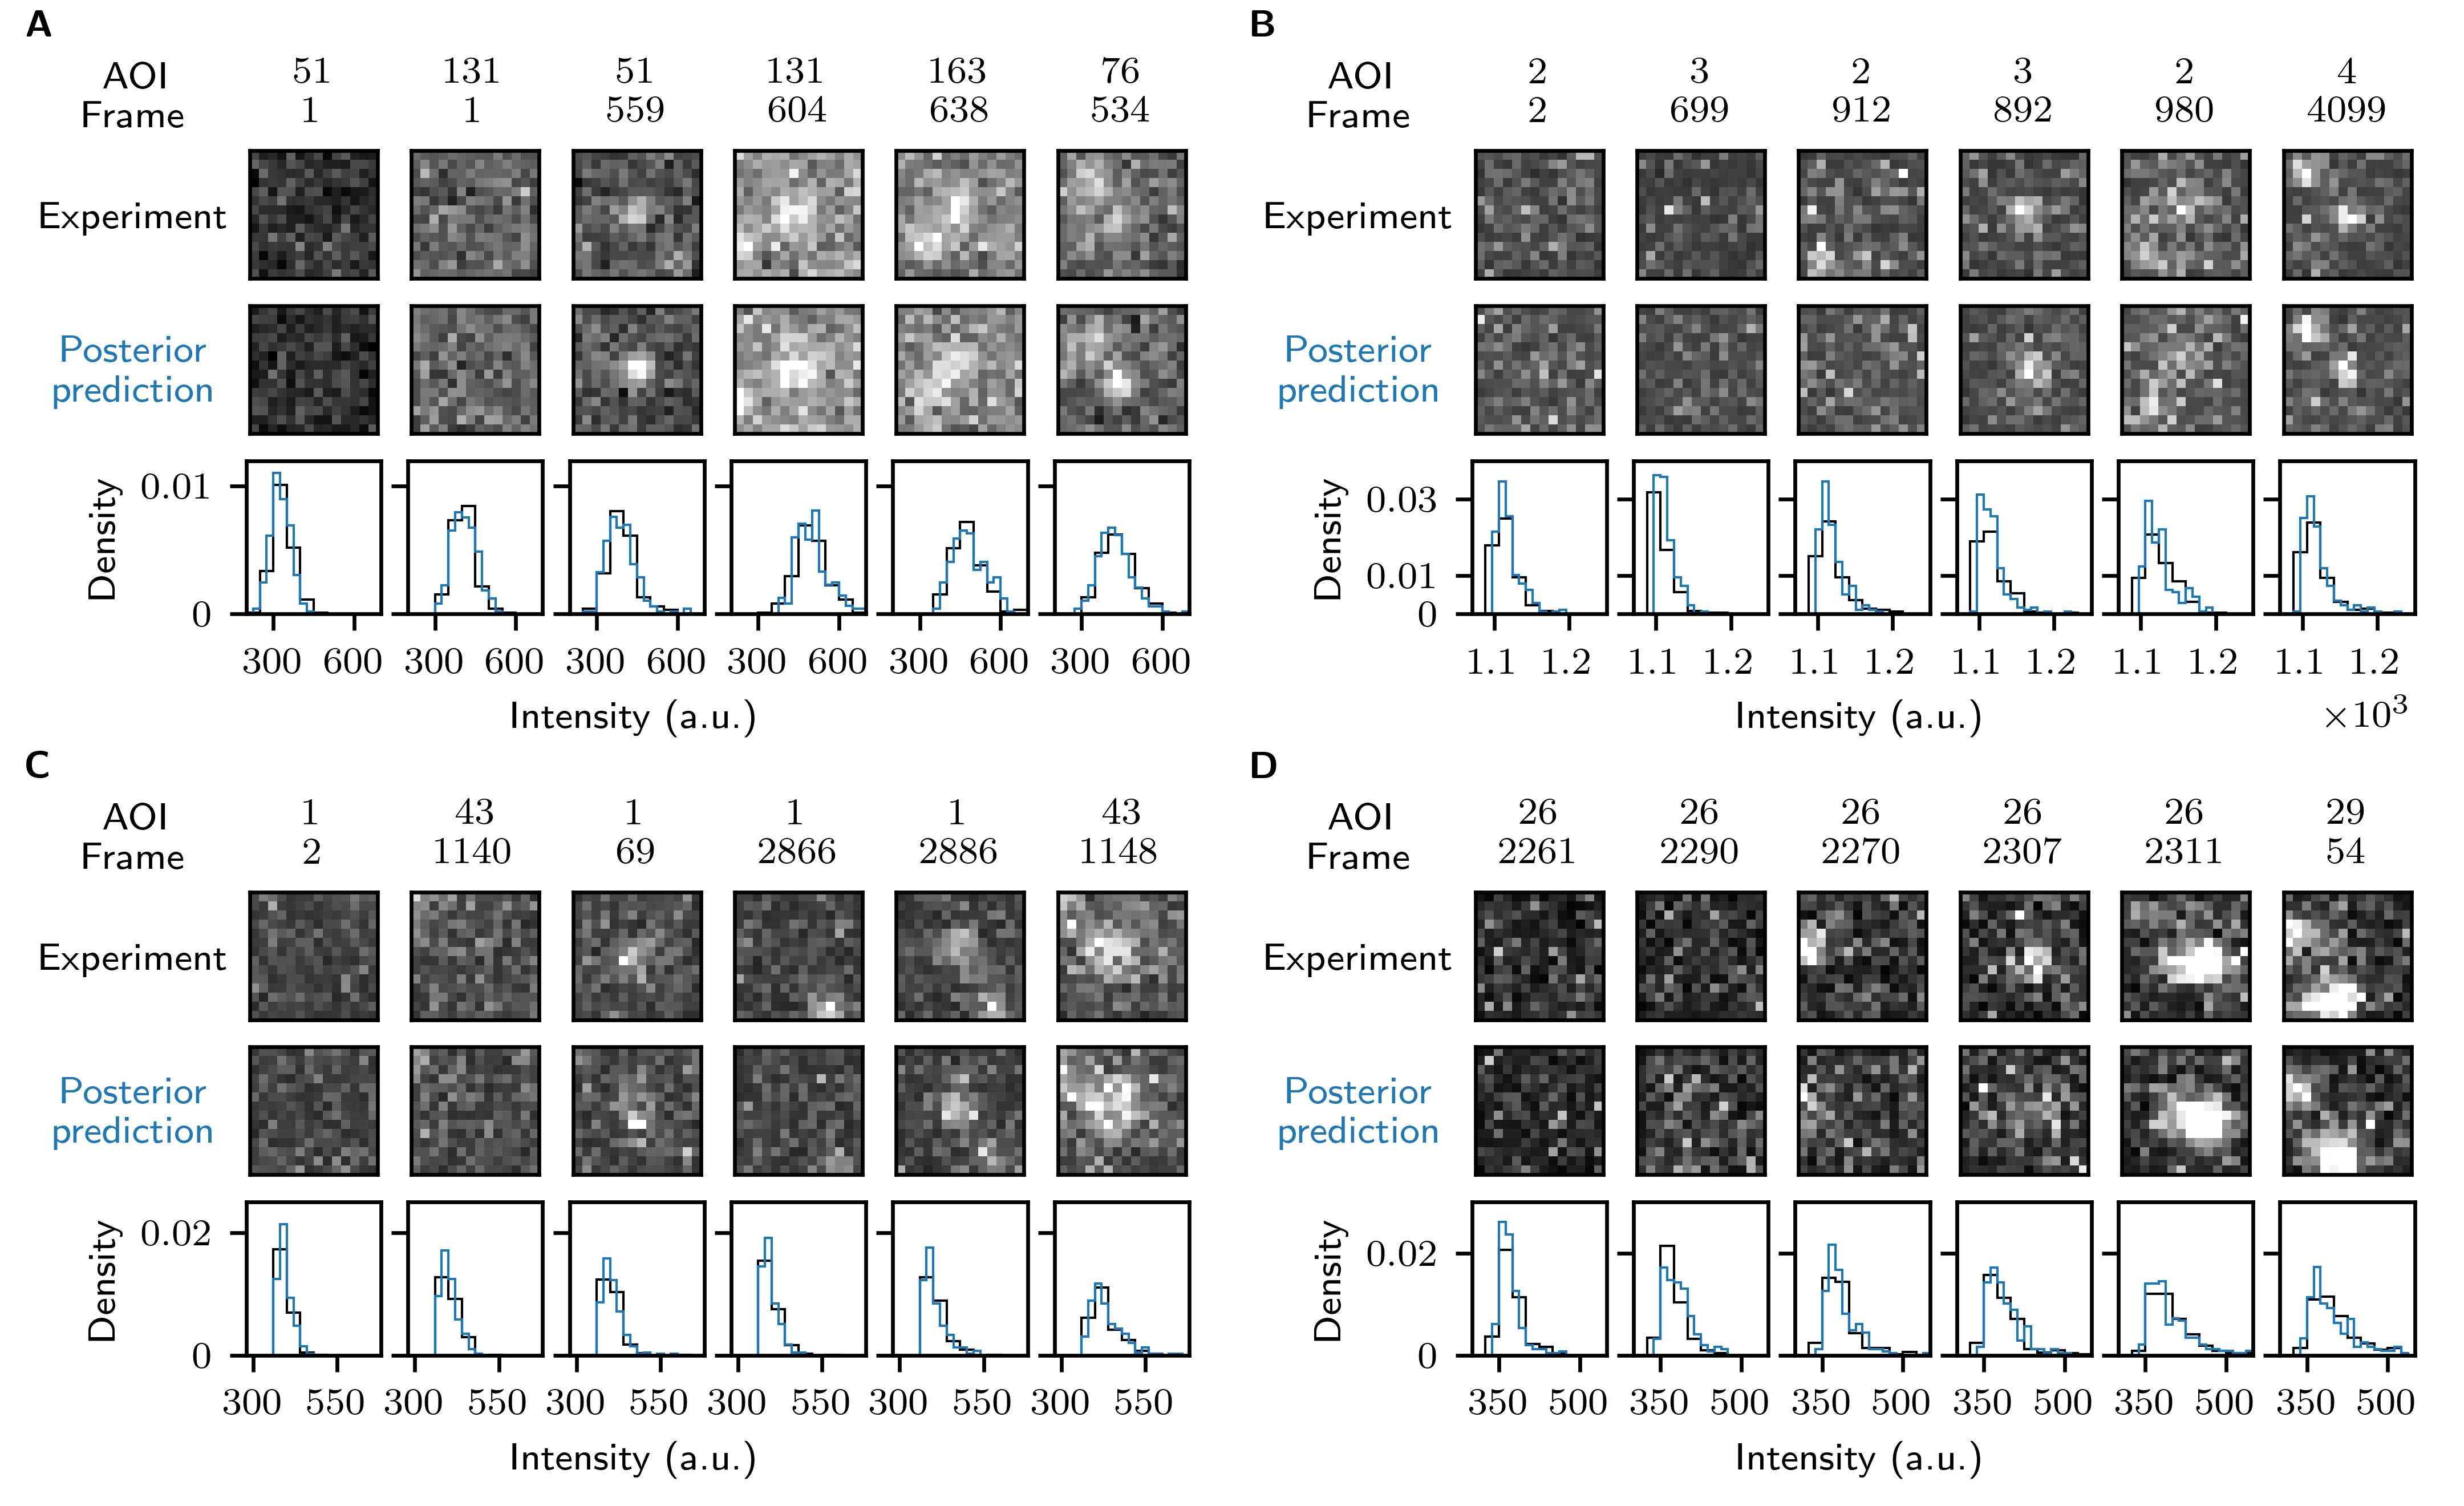
\includegraphics[width=183mm]{figures/tapqir_analysis_ppc.png}}\label{figsupp:ppc}

\figsupp[Tapqir analysis of image data simulated using a broad range of global parameters.]{\textbf{Tapqir analysis of image data simulated using a broad range of global parameters.} Simulations (see Materials and Methods) consist of 16 data sets where values of global parameters ($\pi$, $\lambda$, $\sigma^{xy}$, and $g$) where randomly generated for each data set (Supplemental Data 2). Simulated data were fit with Tapqir, and parameter values from the fit (with 95\% credible interval estimated from a sample size of 10,000) are plotted against the true parameter values. To guide the eye, dashed lines  indicate identical true and fit values. (\textbf{A}) Gain of the camera $g$. (\textbf{B}) Average target-specific binding probability $\pi$. (\textbf{C}) Target non-specific binding density $\lambda$. (\textbf{D}) Proximity parameter $\sigma^{xy}$.}{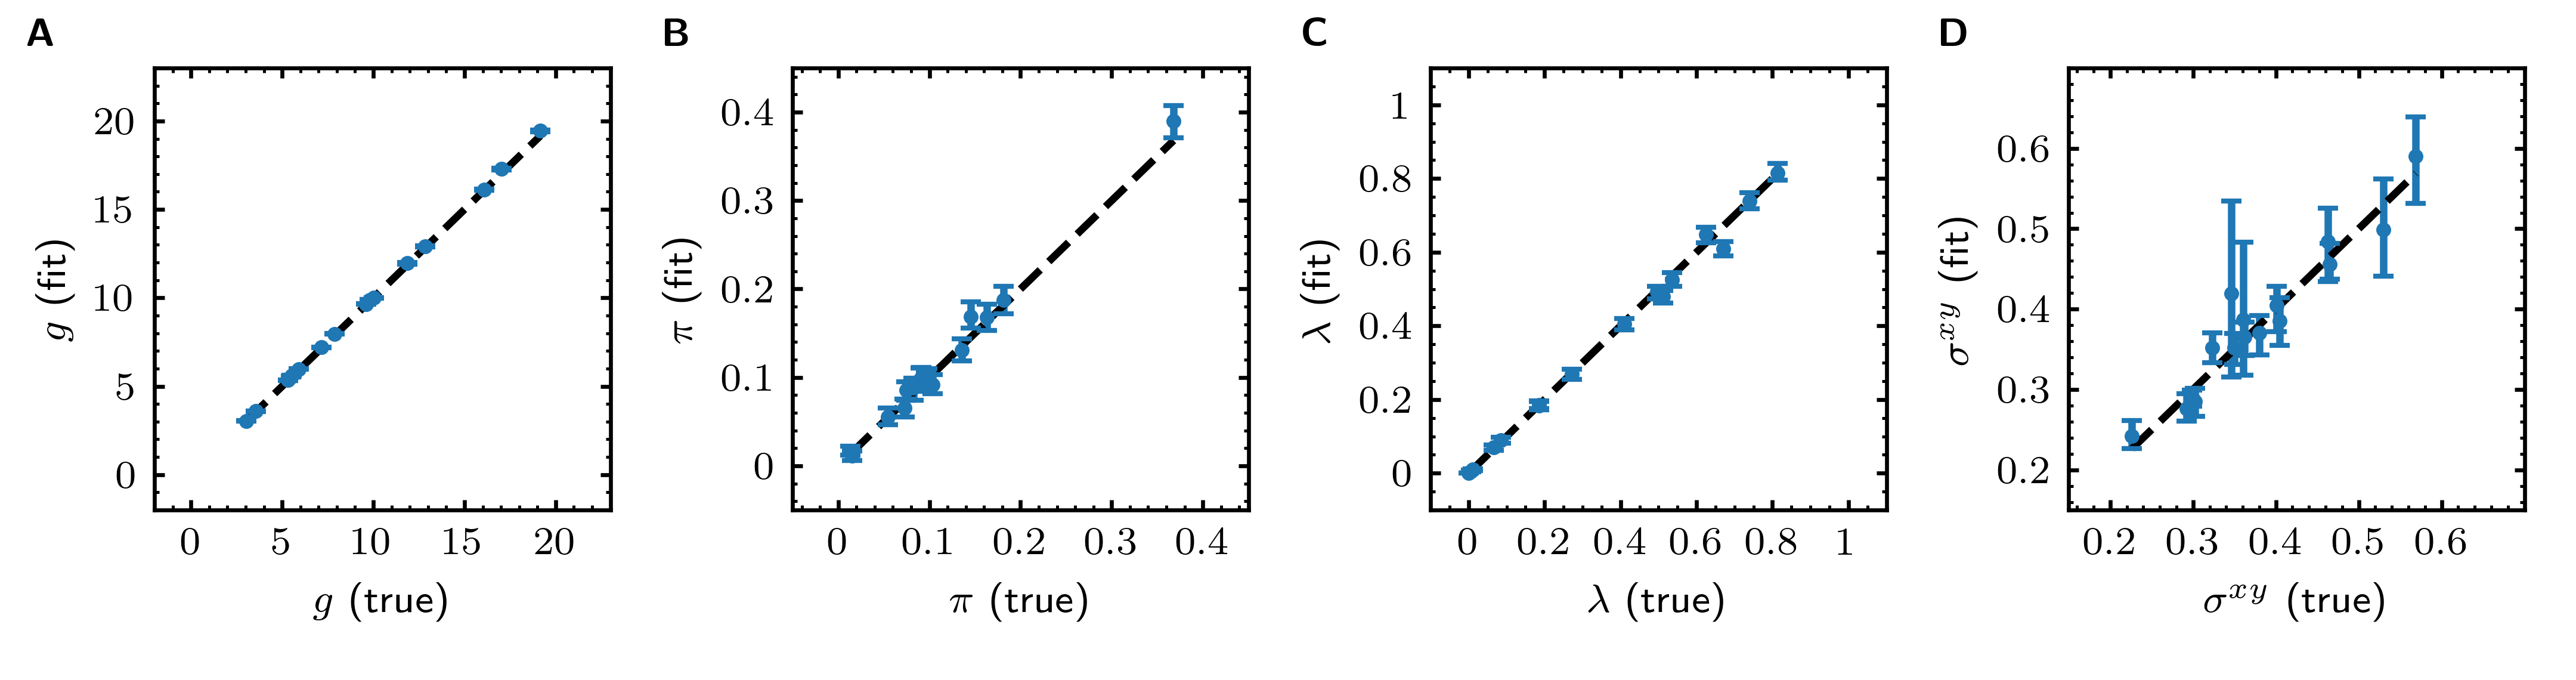
\includegraphics[width=183mm]{figures/tapqir_analysis_randomized.png}}\label{figsupp:randomized}

\figsupp[Effect of AOI size on analysis of experimental data.]{\textbf{Effect of AOI size on analysis of experimental data.} (\textbf{A}) and (\textbf{B}) each show a short extract from a single target location (AOI 163 in (\textbf{A}) and AOI 0 in (\textbf{B})) from Data set A (\TABLE{datasets}; SNR = 1.61). Tapqir was applied to the data set using AOI image sizes $P$ of $14 \times 14$ (first row), $10 \times 10$ (second row), and $6 \times 6$ (third row) pixels. Corresponding output $p(\mathsf{specific})$ probabilities are plotted in the graph. Image contrasts in (\textbf{A}) and (\textbf{B}) are different. Unattended calculation time on an AMD Ryzen Threadripper 2990WX with an Nvidia GeForce RTX 2080Ti GPU using CUDA version 11.5 for the different AOI sizes were: 7 h 40 min ($P=14$), 3 h 5 min ($P=10$), and 2 h 40 min ($P=6$).}{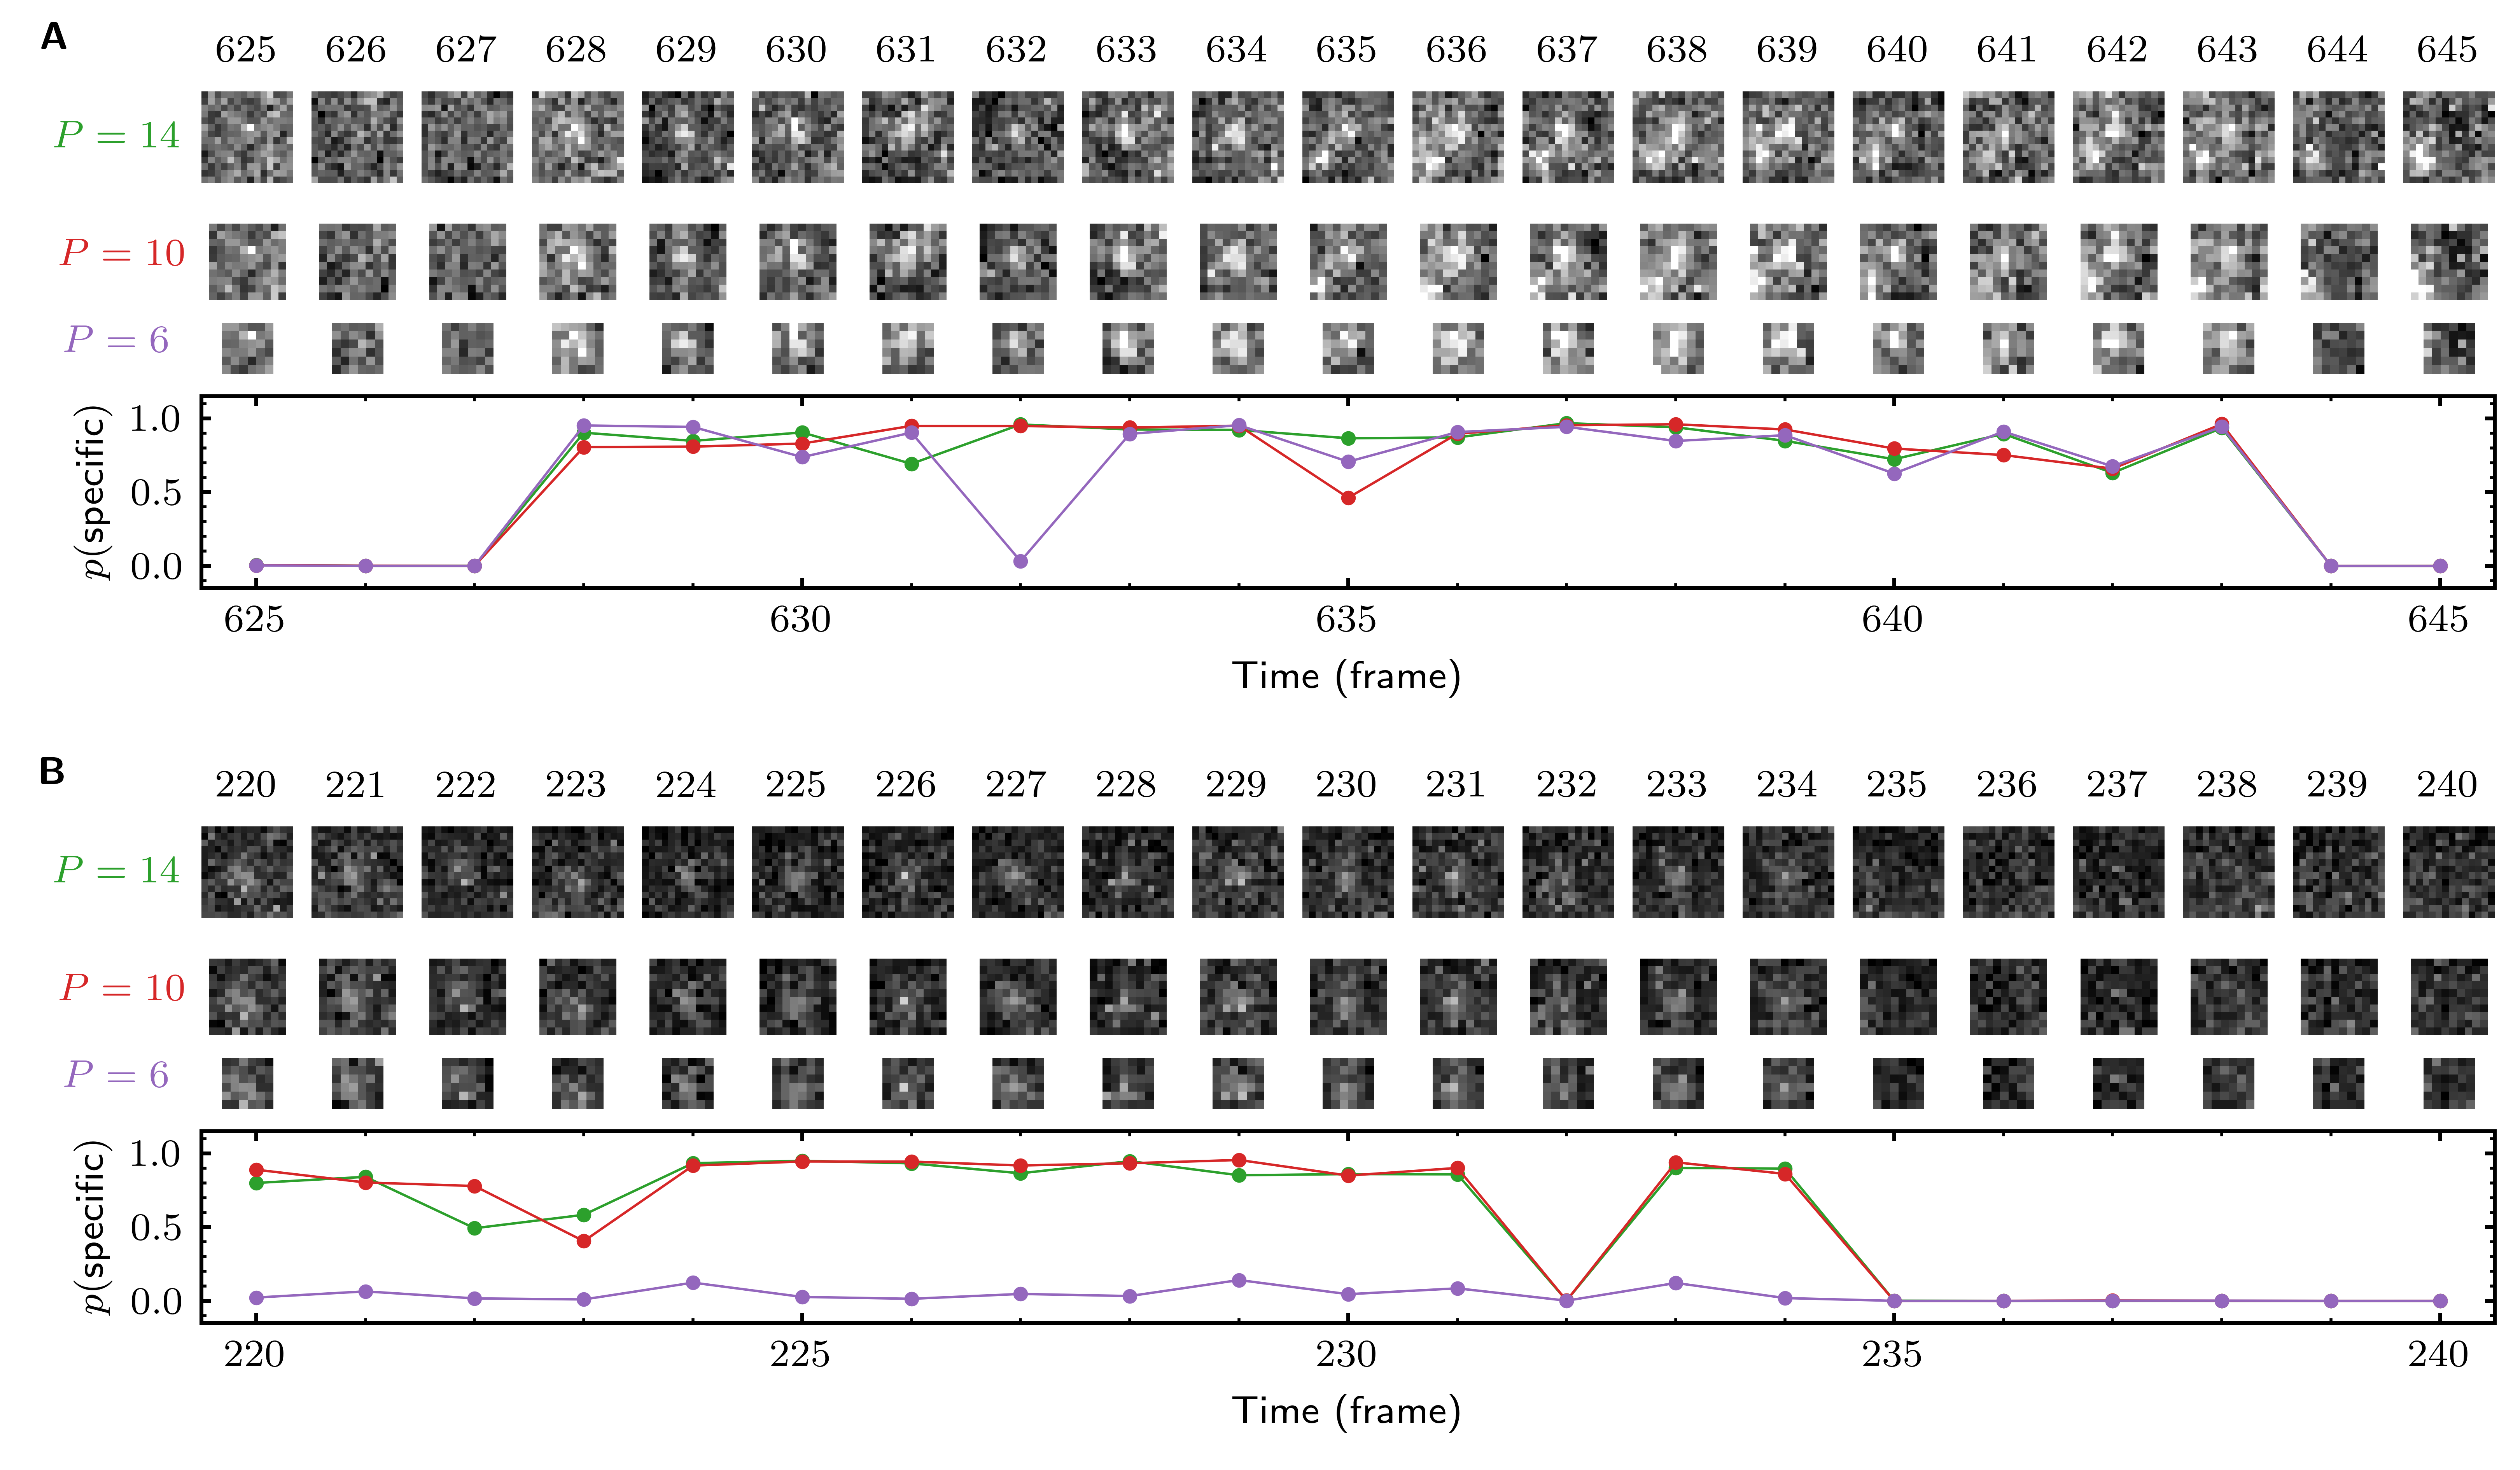
\includegraphics[width=183mm]{figures/tapqir_analysis_size.png}}\label{figsupp:size}
\end{fullwidth}
\end{figure}